\documentclass{article}

\usepackage{neurips_2023}



\usepackage[utf8]{inputenc} % allow utf-8 input
\usepackage[T1]{fontenc}    % use 8-bit T1 fonts
\usepackage{hyperref}       % hyperlinks
\usepackage{url}            % simple URL typesetting
\usepackage{booktabs}       % professional-quality tables
\usepackage{amsfonts}       % blackboard math symbols
\usepackage{nicefrac}       % compact symbols for 1/2, etc.
\usepackage{microtype}      % microtypography
\usepackage{xcolor}         % colors
\usepackage{graphicx}
\graphicspath{ {./imagenes/} }

\title{Pre TP1: Data Mining en Ciencia y Tecnología}

\author{%
  José Saint Germain\\
  \texttt{josesg998@gmail.com} \\
}

\begin{document}

\maketitle

\section{Introducción}

El procesamiento de imágenes resulta desafiante por su alta 
dimensionalidad. La estructura de una {\bf imagen digital} consiste 
en una  {\bf matriz de NxM}, en donde la subunidad constituyente de 
la matriz es un  {\bf pixel} que codifica información para un color 
particular. Cada pixel representa la intesidad de luz en ese 
punto, que generalmente varía entre  {\bf [0,255]}, 
lo que es equivalente a  {\bf8 bits.}\

Para representar imágenes a colores, se utiliza un modelo de 
percepción humana, en donde el color resulta a través de un
sistema aditivo. El modelo se basa en la teoría de los componentes
primarios del color que son Rojo, Verde y Azul  {\bf (RGB Red, Green 
and Blue}, por sus siglas en inglés). Por consiguiente, para 
representar digitalmente una imagen color, se necesitan  {\bf 3 
matrices de NxM}. Una para el Rojo, otra para el Verde y 
otra para el Azul.

\section{Objetivos}


Familiarizarse con el procesamiento de imágenes. Para ello, se proponen 
diferentes manipulaciones que permitirán preparar el dataset para la 
detección y exploración de agrupamientos naturales.

\section{Estructura de los datos}

A partir del siguiente \href{https://www.kaggle.com/datasets/olgabelitskaya/flower-color-images}{link},
se obtendrán las imágenes a color de {\bf 210 flores} pertenecientes a {\bf 10 especies 
diferentes}. Cada imagen consiste en un archivo {\bf .PNG} de 128 pixeles de ancho 
por 128 pixeles de profundidad ({\bf 128x128x3}). Adicionalamente, se encuentra el 
archivo {\bf .CSV} con las etiquetas (labels) que corresponden a la especie de cada imagen.

\section{Procesamiento de imágenes}

{\emph Cargar el dataset de imágenes y sus respectivas etiquetas. Es importante asegurarse que las 
imágenes sean comparables en color, valor, rango y tamaño.

Explorar y graficar los subconjuntos de imágenes que representan flores de la misma
especie.}
\pagebreak

En el siguiente gráfico, se tomó una muestra de cuatro flores por especie:

\begin{figure}[h!]
  \centering  
  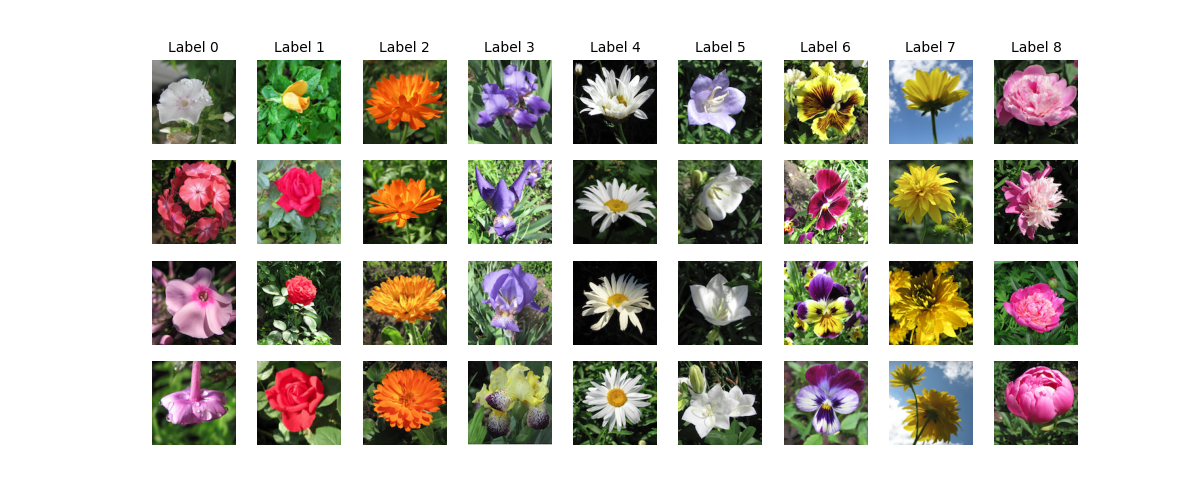
\includegraphics[width=1\textwidth]{1_ejemplos_flores.png}
  \caption{Exploración de especies de flores}
\end{figure}

Analizando todos los archivos noté que la imagen '00218.png'
tiene una resolución mayor a la del resto, lo cual 
puede dificultar algunos análisis como el cálculo de una imagen. Por lo tanto,
se decidió quitar la imagen del análisis.

\section{Manipulación de datos}

\subsection{Cambio de brillo}

{\emph Cambiar la intensidad de una de las imágenes en escala de grises, transformarla en una imagen con mucho y otra con poco brillo.}

\begin{figure}[h!]
  \centering    
  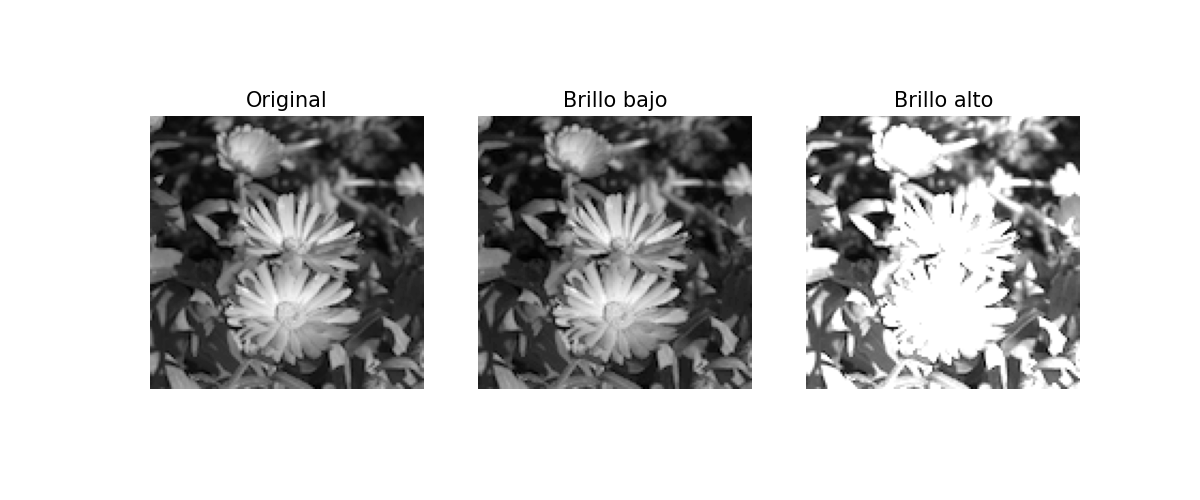
\includegraphics[width=1\textwidth]{2_brillo.png}
  \caption{Ajuste de brillo}
\end{figure}

\subsection{Imagen en blanco y negro}

{\emph Convertir una de las imágenes a blanco y negro (binario). ¿Es la única manera? Si existen otras transformaciones mostrar más de una conversión}
\pagebreak
\begin{figure}[h!]
  \centering    
  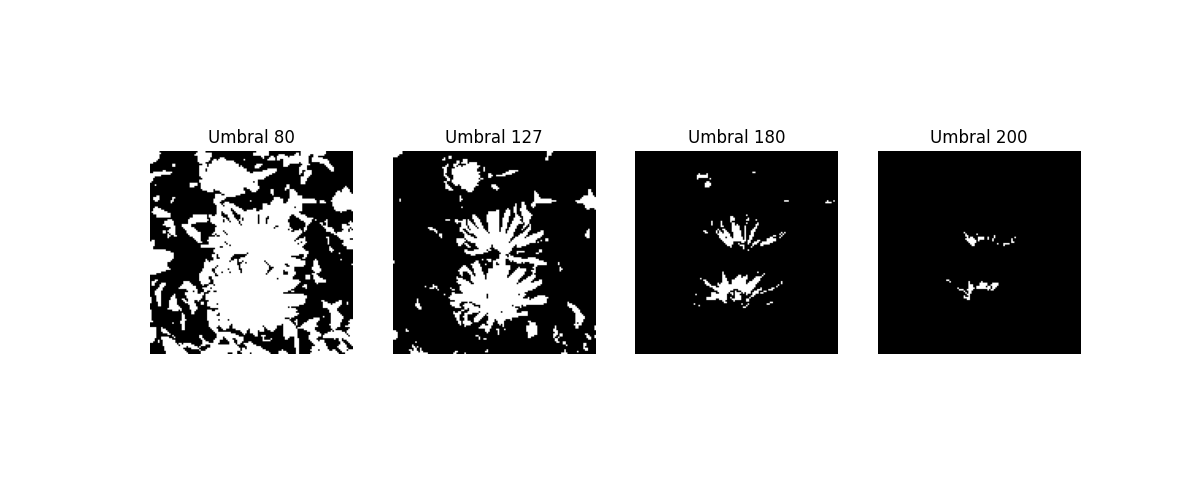
\includegraphics[width=.75 \textwidth]{3_binario.png}
  \caption{Imágenes binarias con disintos umbrales}
\end{figure}

Para pasar una imagen a binaria, es necesario establecer un umbral para el valor del píxel.
De esa manera, cualquier pixel que supere ese umbral será blanco y cualquier pixel que esté por
debajo será negro. A medida que aumentes el umbral, como se ve en las imágenes, una mayor proporción
de los píxeles pasarán a ser negros.

\subsection{Imagen recortada}
\label{others}

{\emph Recortar una parte significativa de la imagen, quedándose sólo con el círculo central de la misma.}

\begin{figure}[h!]
  \centering    
  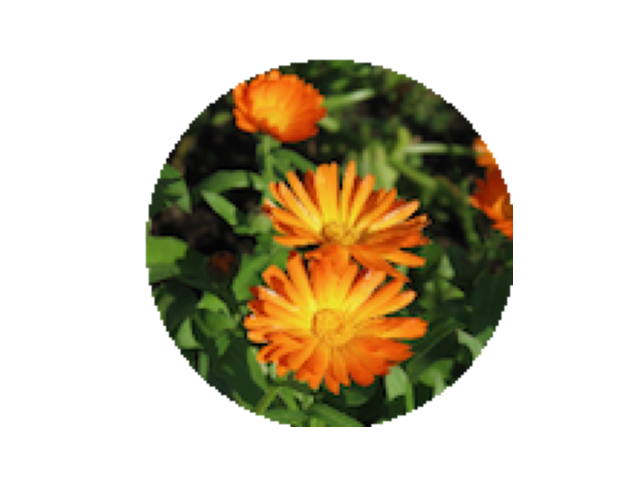
\includegraphics[width=.3\textwidth]{4_recortado.png}
  \caption{Recorte de imagen}
\end{figure}
\subsection{Imágenes mezcladas}

{\emph Generar dos imágenes random: una imagen mezclando los pixels y otra mezclando
partes de diferentes imágenes.}

\begin{figure}[h!]
  \centering    
  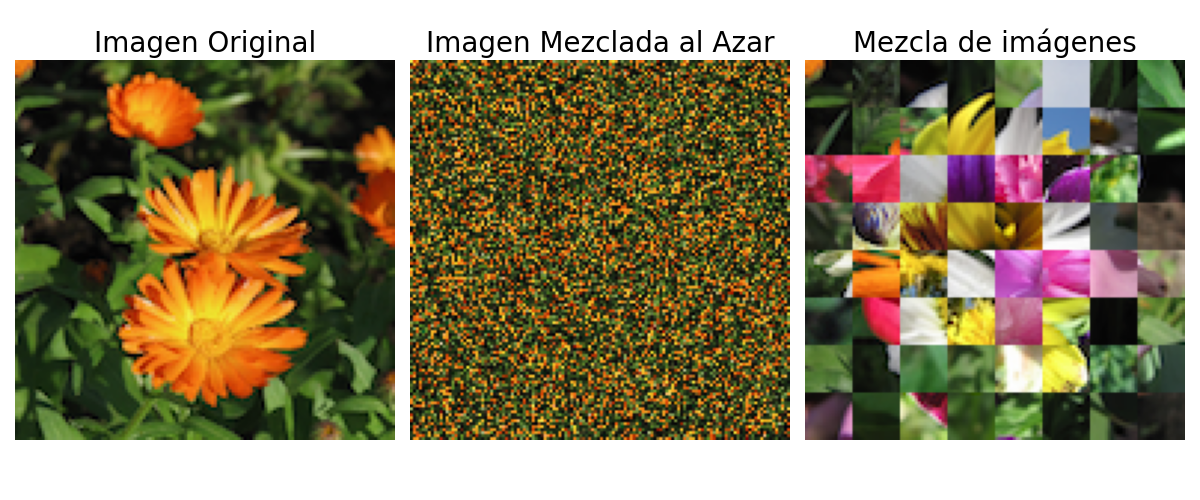
\includegraphics[width=.75\textwidth]{5_mezcla.png}
  \caption{Imagenes con píxeles mezclados e intercambiados}
\end{figure}

Con respecto a la mezcla de imágenes, se puede alterar el tamaño de la porción
de las imágenes, por lo que se podría mezclar cada pixel o bien utilizar
cuadrados más grandes.

\subsection{Filtros de imagen}

{\emph Aplicar dos tipos diferentes de filtros sobre una imagen, 
explique en qué casos conviene usar cada uno.}
\begin{figure}[h!]
  \centering    
  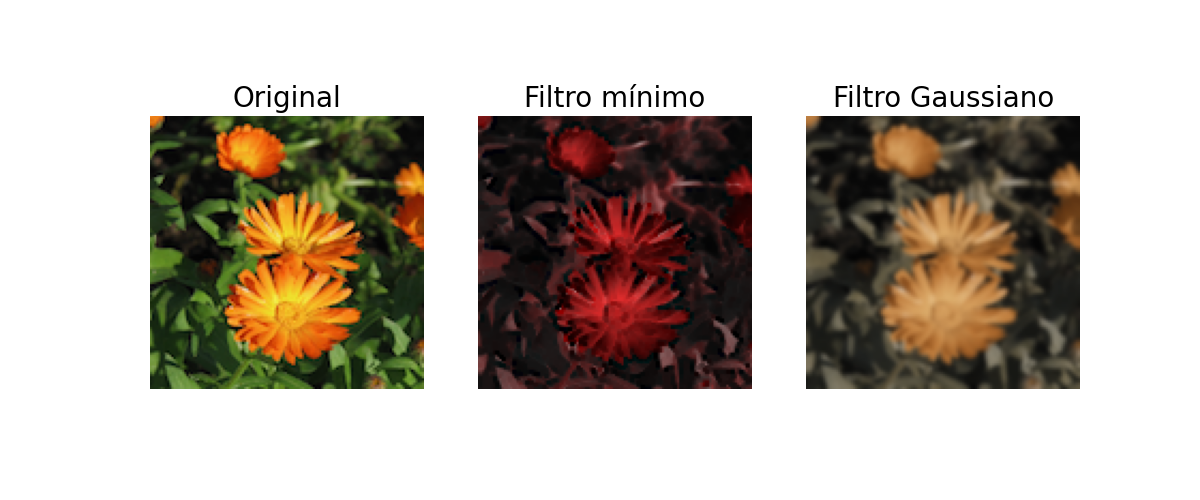
\includegraphics[width=1\textwidth]{6_filtro.png}
  \caption{Imagenes con filtros}
\end{figure}

El filtro mínimo toma una porción de píxeles (en este caso, de tamaño 2) y 
le aplica a todos el valor del píxel mínimo. Se utiliza para remover 
outliers positivos, es decir píxeles de colores claros.

El filtro gaussiano tiene un uso similar al mean filter, con la
diferencia de que el primero tiene en cuenta la distancia de los 
píxeles a los que se les aplica el filtro. De esa manera, los píxeles
más cercanos al centro del conjunto de píxeles (en este caso se seleccionó un
desvío estándar de 1) tienen mayor peso que los lejanos. Se suele preferir
frente al medio cuando se quiere suavizar la imagen pero sin transiciones
fuertes entre los píxeles.

\subsection{Imágenes promedio}

{\emph Calcular imagen promedio global y el promedio entre las distintas especies. ¿Se pueden
distinguir los promedios? ¿Cómo quedan los promedios si consideran las imágenes en
blanco y negro?}

\begin{figure}[h!]
  \centering    
  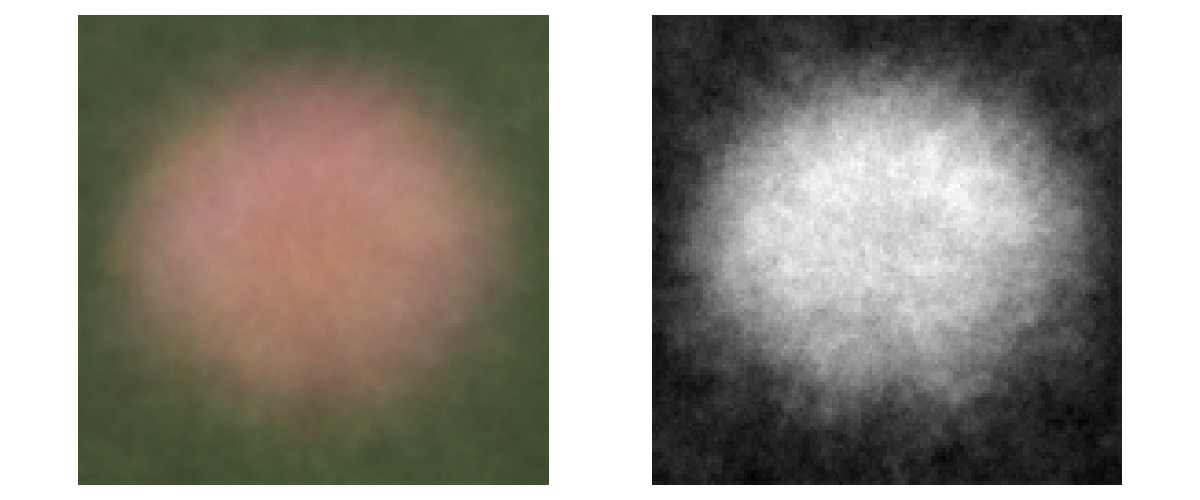
\includegraphics[width=.7\textwidth]{7_1_promedio.png}
  \caption{Imagenes promedio color y blanco y negro}
\end{figure}


\begin{figure}[h!]
  \centering    
  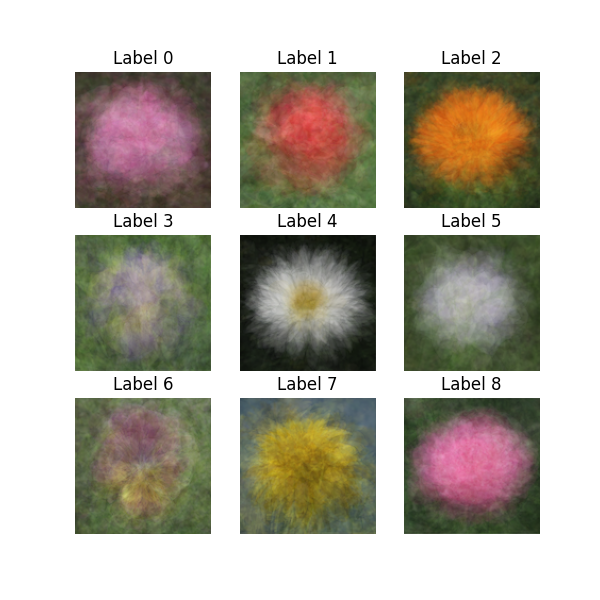
\includegraphics[width=.6\textwidth]{7_2_promedio_especies_color.png}
  \caption{Imagenes promedio color}
\end{figure}

\begin{figure}[h!]
  \centering    
  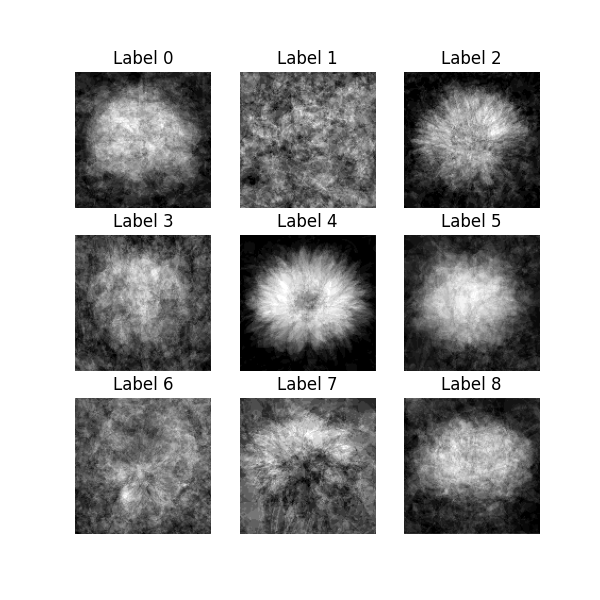
\includegraphics[width=.6\textwidth]{7_3_promedio_especies_bn.png}
  \caption{Imagenes promedio blanco y negro}
\end{figure}
\pagebreak
Las imágenes promedio en color permiten distinguirlas facilmente. Incluso,
en el caso de la especie 4, permite identificar de forma bastante precisa sus
características. En el resto se puede apreciar el rango de color en el que se
manejan sus pétalos. Las imágenes en blanco y negro, en cambio, dificultan identificar diferencias
entre especies, a excepción de la especie 4. En la especie 1 ni siquiera se
puede identificar la flor con respecto al fondo. Es posible que modificando el
umbral se logre distinguir mejor otras especies.

\section{Búsqueda de features}

{\emph Analizar las distribuciones de valores de pixels por cada especie. ¿Se puede distinguir
una especie en algún rango de color?}

\begin{figure}[h!]
  \centering    
  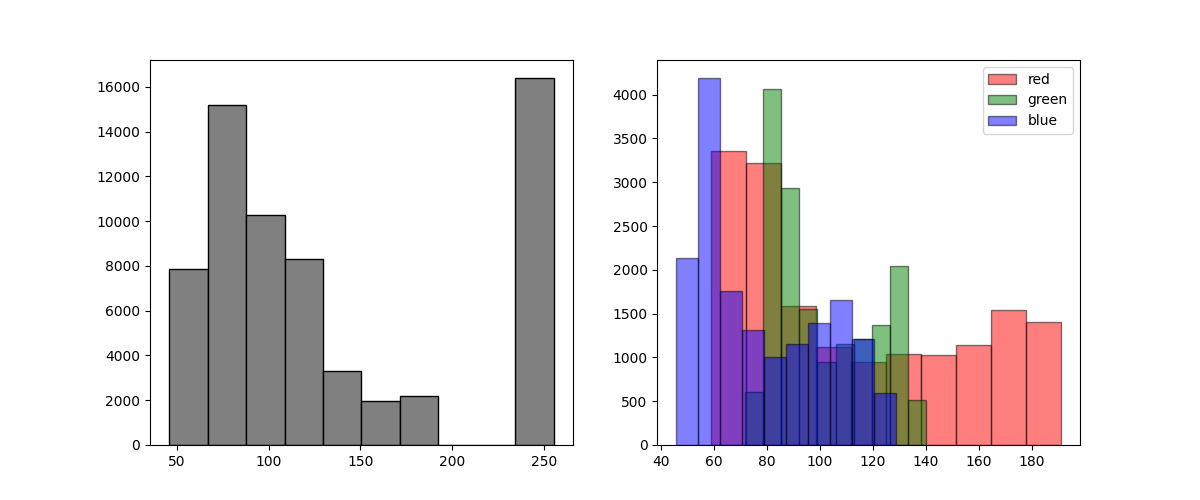
\includegraphics[width=.75\textwidth]{8_1_pixeles_general.png}
  \caption{Distribución promedio de píxeles}
\end{figure}

% \begin{figure}[h!]
%   \centering    
%   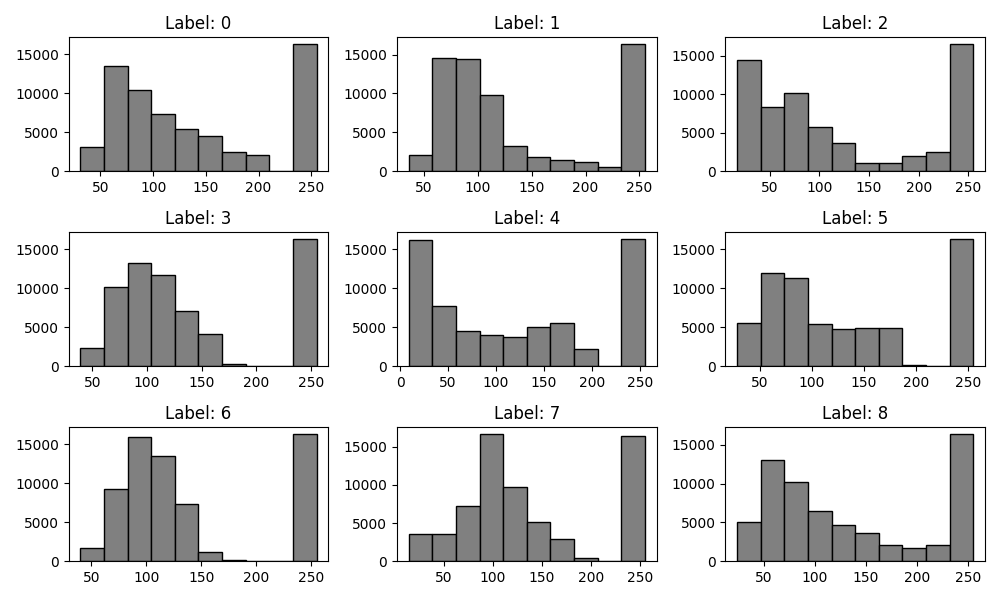
\includegraphics[width=1\textwidth]{8_2_pixeles_especies_byn.png}
%   \caption{Distribución de pixeles por especie}
% \end{figure}

\begin{figure}[h!]
  \centering    
  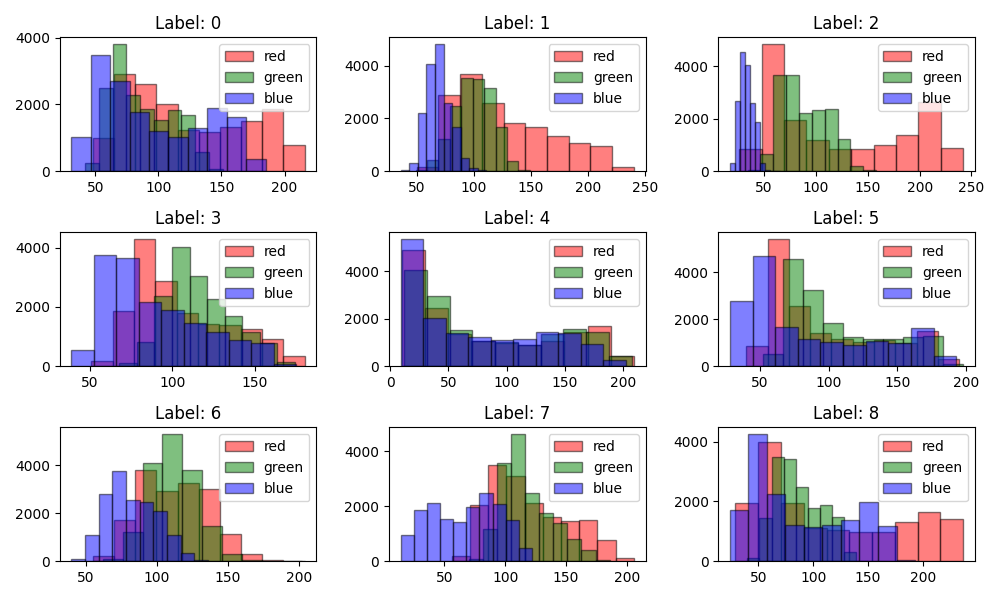
\includegraphics[width=1\textwidth]{8_3_pixeles_especies_color.png}
  \caption{Distribución de pixeles de color por especie}
\end{figure}

Para este análisis, es muy útil referenciarse con las imágenes promedio.
Por ejemplo, la imagen promedio global contiene una gran cantidad de píxeles
rojos, lo cual se evidencia en su aspecto rosado. Interesantemente, la especie
8 mantiene una distribución similar, lo cual se evidencia en que su promedio
también es rosado. Otra especie a destacar es la 4, puesto que la distribución
de los tres colores es casi idéntico, expresándose en sus pétalos blancos.
\pagebreak

\subsection{Análisis de componentes principales}

{\emph Realizar una inspección de las componentes principales del dataset y analizar si se
pueden identificar las especies en esta representación.}

Una vez realizado el análisis de componentes principales, se midió y graficó la
varianza explicada acumulada de cada componente. Como se ve en el gráfizo de la
izquierda, los primeros 2 componentes explican el 20 por ciento de la varianza,
lo cual es un valor bastante bajo para realizar un análisis significativo.
Adicionalmente,  si quisiéramos explicar al menos el 70 por ciento de la varianza,
necesitaríamos un poco menos de 50 componentes.

Esta conclusión se refuerza con el gráfico de la derecha, en donde se utilizan
los primeros dos componentes y se colorean los puntos con la especie correspondiente.
Como se puede apreciar, no se puede distinguir ningún grupo de puntos de un color
particular.

\begin{figure}[h!]
  \centering    
  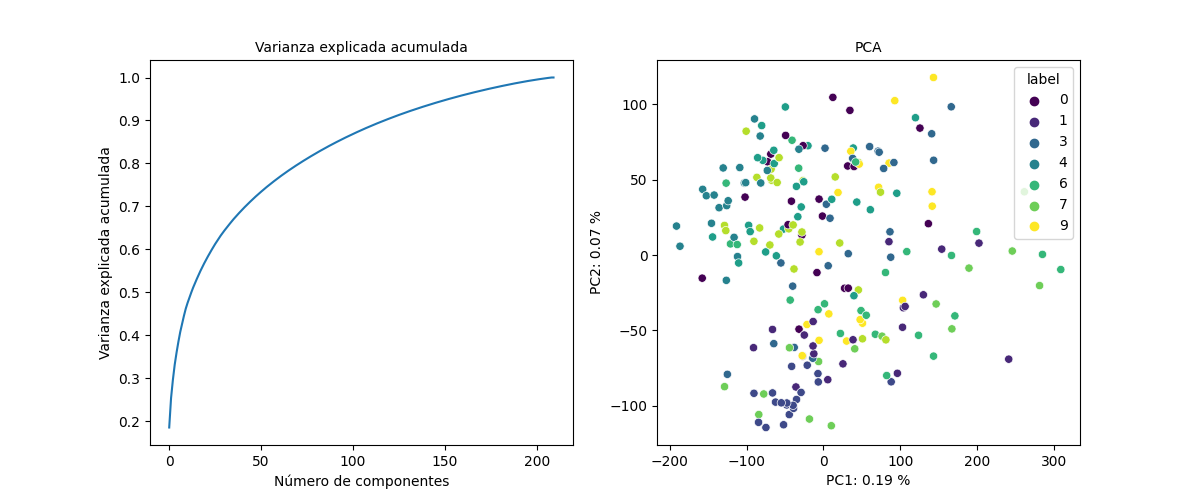
\includegraphics[width=1\textwidth]{9_1_pca.png}
  \caption{Análisis de componentes principales}
\end{figure}

%%%%%%%%%%%%%%%%%%%%%%%%%%%%%%%%%%%%%%%%%%%%%%%%%%%%%%%%%%%%


\end{document}